\documentclass[tikz,border=0pt]{standalone}
\usepackage[utf8]{inputenc}
\usepackage[T1]{fontenc}
\usepackage{lmodern}
\usepackage{amsmath,amssymb}
\usetikzlibrary{arrows.meta,positioning,fit,calc,backgrounds,shapes.geometric,decorations.pathreplacing}
\definecolor{navy}{HTML}{163A5F}
\definecolor{blue}{HTML}{2C6EAF}
\definecolor{lightblue}{HTML}{EAF2F8}
\definecolor{midblue}{HTML}{CFE1F2}
\definecolor{graytext}{HTML}{4A5560}
\definecolor{lightgray}{HTML}{F4F6F8}
\definecolor{green}{HTML}{3C8D73}
\definecolor{lightgreen}{HTML}{E8F5EF}
\definecolor{red}{HTML}{B24A4A}
\definecolor{lightred}{HTML}{FBEDEE}
\tikzset{
  title/.style={font=\sffamily\bfseries\fontsize{16}{18}\selectfont,text=navy,anchor=west},
  subtitle/.style={font=\sffamily\bfseries\fontsize{11}{13}\selectfont,text=navy},
  body/.style={font=\sffamily\fontsize{9.2}{11}\selectfont,text=graytext,align=left},
  small/.style={font=\sffamily\fontsize{8}{9.4}\selectfont,text=graytext,align=left},
  tinylabel/.style={font=\sffamily\fontsize{7.2}{8.4}\selectfont,text=graytext},
  panel/.style={rounded corners=3pt,draw=midblue,fill=white,line width=0.6pt},
  box/.style={rounded corners=2pt,draw=midblue,fill=lightblue,line width=0.6pt},
  worker/.style={rounded corners=2pt,draw=blue,dashed,line width=0.7pt,fill=white},
  task/.style={rounded corners=2pt,draw=blue,fill=lightblue,minimum width=0.85cm,minimum height=0.55cm,font=\sffamily\bfseries\small,text=navy},
  file/.style={draw=blue,fill=white,minimum width=0.55cm,minimum height=0.42cm,font=\sffamily\small,text=navy},
  arr/.style={-{Stealth[length=2.4mm,width=1.8mm]},draw=blue,line width=0.9pt},
  arrthin/.style={-{Stealth[length=2mm,width=1.5mm]},draw=blue,line width=0.7pt},
  arrred/.style={-{Stealth[length=2mm,width=1.5mm]},draw=red,dashed,line width=0.8pt},
  arrgreen/.style={-{Stealth[length=2mm,width=1.5mm]},draw=green,dotted,line width=1pt}
}
\begin{document}

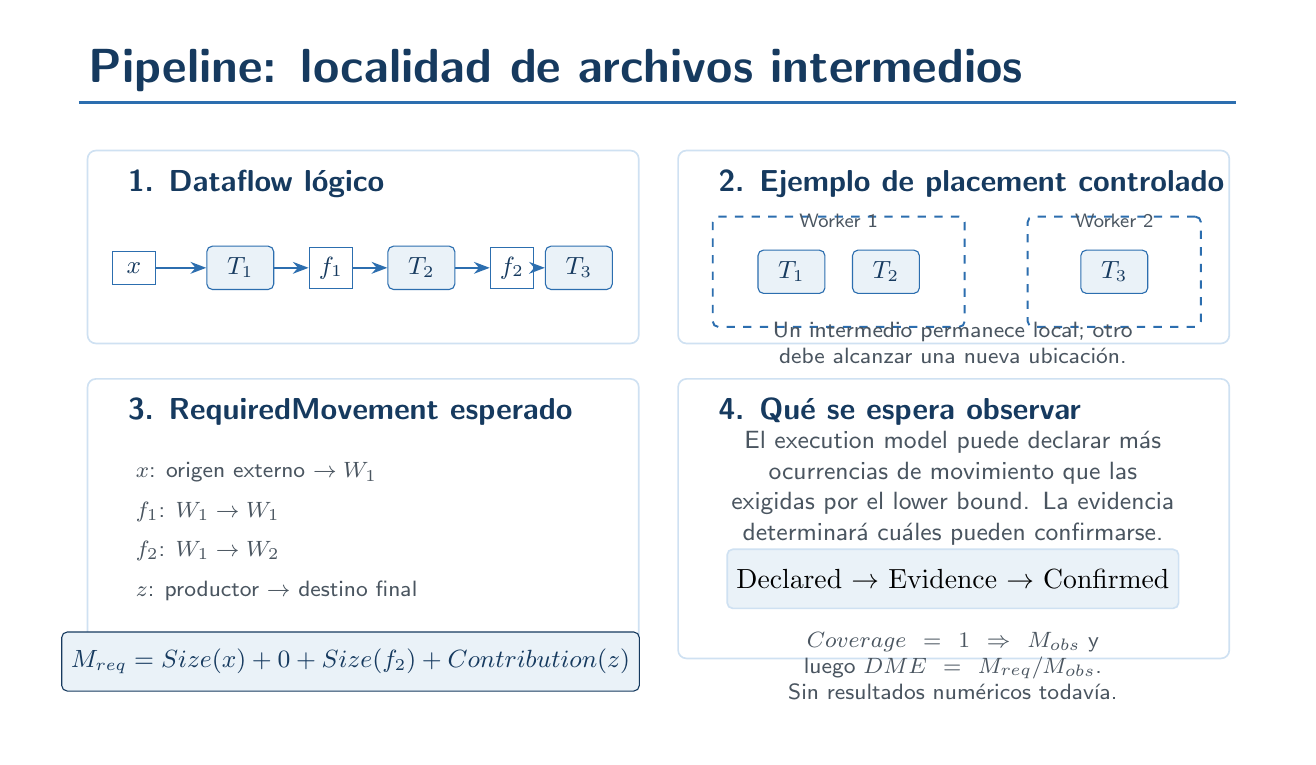
\begin{tikzpicture}[x=1cm,y=1cm]
\path[use as bounding box] (0,0) rectangle (16,9);
\node[title] at (0.65,8.45) {Pipeline: localidad de archivos intermedios};
\draw[blue,line width=1pt] (0.65,8.05)--(15.35,8.05);
\node[panel,minimum width=7cm,minimum height=2.45cm,anchor=north west] at (0.75,7.45) {};
\node[subtitle,anchor=west] at (1.15,7.02) {1. Dataflow lógico};
\node[file] (x) at (1.35,5.95) {$x$}; \node[task] (t1) at (2.7,5.95) {$T_1$}; \node[file] (f1) at (3.85,5.95) {$f_1$}; \node[task] (t2) at (5.0,5.95) {$T_2$}; \node[file] (f2) at (6.15,5.95) {$f_2$}; \node[task] (t3) at (7.0,5.95) {$T_3$};
\draw[arrthin] (x)--(t1); \draw[arrthin] (t1)--(f1); \draw[arrthin] (f1)--(t2); \draw[arrthin] (t2)--(f2); \draw[arrthin] (f2)--(t3);
\node[panel,minimum width=7cm,minimum height=2.45cm,anchor=north west] at (8.25,7.45) {};
\node[subtitle,anchor=west] at (8.65,7.02) {2. Ejemplo de placement controlado};
\node[worker,minimum width=3.2cm,minimum height=1.4cm] at (10.3,5.9) {}; \node[worker,minimum width=2.2cm,minimum height=1.4cm] at (13.8,5.9) {};
\node[tinylabel] at (10.3,6.55) {Worker 1}; \node[tinylabel] at (13.8,6.55) {Worker 2};
\node[task] at (9.7,5.9) {$T_1$}; \node[task] at (10.9,5.9) {$T_2$}; \node[task] at (13.8,5.9) {$T_3$};
\node[small,text width=5.7cm,align=center] at (11.75,5.0) {Un intermedio permanece local; otro debe alcanzar una nueva ubicación.};
\node[panel,minimum width=7cm,minimum height=3.55cm,anchor=north west] at (0.75,4.55) {};
\node[subtitle,anchor=west] at (1.15,4.12) {3. RequiredMovement esperado};
\node[small,anchor=west] at (1.25,3.35) {$x$: origen externo $\rightarrow W_1$};
\node[small,anchor=west] at (1.25,2.85) {$f_1$: $W_1\rightarrow W_1$};
\node[small,anchor=west] at (1.25,2.35) {$f_2$: $W_1\rightarrow W_2$};
\node[small,anchor=west] at (1.25,1.85) {$z$: productor $\rightarrow$ destino final};
\node[rounded corners=2pt,draw=navy,fill=lightblue,minimum width=5.6cm,minimum height=0.75cm,font=\sffamily\bfseries\small,text=navy] at (4.1,0.95) {$M_{req}=Size(x)+0+Size(f_2)+Contribution(z)$};
\node[panel,minimum width=7cm,minimum height=3.55cm,anchor=north west] at (8.25,4.55) {};
\node[subtitle,anchor=west] at (8.65,4.12) {4. Qué se espera observar};
\node[body,text width=5.8cm,align=center] at (11.75,3.15) {El execution model puede declarar más ocurrencias de movimiento que las exigidas por el lower bound. La evidencia determinará cuáles pueden confirmarse.};
\node[box,minimum width=5.0cm,minimum height=0.75cm] at (11.75,2.0) {Declared $\rightarrow$ Evidence $\rightarrow$ Confirmed};
\node[small,text width=5.6cm,align=center] at (11.75,0.9) {$Coverage=1 \Rightarrow M_{obs}$ y luego $DME=M_{req}/M_{obs}$. Sin resultados numéricos todavía.};
\end{tikzpicture}
\end{document}
